\documentclass[12pt, draft]{article}
\usepackage{candor, setspace, wrapfig}
\newcommand{\BWFtitle}{Computationally Modeling Ribosomal Translation
    and Programmed Frameshifts in}

\usepackage[final, colorlinks=true, linkcolor=BWFBlue,
  citecolor=BWFGreen, urlcolor=BWFRed, pdftitle={\BWFtitle Escherichia
    coli}, pdfauthor={Hao Lian, Vivek Bhattacharya, and Daniel Vitek},
  pdfsubject={Bioinformatics, Genetics, and Biology}, pdfcreator={The
    Frameshift Kids}, pdfkeywords={bioinformatics,genetics,biology,
    frameshifts,perl,matlab,ecoli,prfb,rpos,bgh}, pdfstartview={FitH},
  backref]{hyperref}

\linespread 2
\numberwithin{equation}{section}

\author{{\sc Hao Lian, Vivek Bhattacharya, and Daniel Vitek}}
\date{{\sc \today}}
\title{\bf{\BWFtitle~\emph{Escherichia coli}}}

\begin{document}
\pagenumbering{roman}
\maketitle
\tableofcontents
\clearpage

\begin{abstract}\begin{normalsize}
  In this document, we discuss a stochastic model for ribosomal displacement relative to reading 
  frame based on forces arising from changes in free energy present in hybridization between the 
  16S rRNA tail and nucleotides upstream from the A-site.  We present both our investigation and 
  potential applications for this model, including optimization of economically significant gene
  sequences such as bovine growth hormone, non-experimental prediction of translational efficiency for man-made 
  proteins, adjustment of calculated tRNA availability values, and modelling of frameshifts in \prfB\ in \ecoli.
  We present this investigation as a series of various inquiries made 
  in subjects ranging throughout the field of molecular biology.  We also applied our stochastic 
  model to create a short, 16-codon sequence that is not known to produce a frameshift in nature 
  in order to test our model's predictive power for synthesized mRNA sequences, and designed an 
  experiment to verify this frameshift.  We expect results in October 2007.
\end{normalsize}\end{abstract}

\clearpage
\pagenumbering{arabic}

\section{Computational Methods}
\subsection{Free Energy}
\label{freeenergy}

Free energy in a cell arises from the hybridization between two
sequences of RNA and drives ribosomal translation~\cite{starmer}.
\citet{weiss88} suggest the 16S tail of the ribosome hybridizes with its mRNA strand;
from this, we can calculate the free energy values for the interaction between the two strands of RNA.
\citet{freier} propose a thermodynamic model for exactly this,
modeling the interaction in terms of \emph{doublets}, which are pairs of consecutive nucleotides.
Using this model, Freier calculated the free energy available
for the hybridization of permutations of RNA doublets.

\subsection{The Deterministic Model}
\citet{lalit:mechanics} assume a sinusoidal model for
free energy, whence we can project free energy onto magnitude and
phase through a memory model. Ponnala simulates free
energy in a memory structure that can store three values (registers)
that he later can represent as a phasor, a concept from physics. Then,
we can visualize free energy from polar plots and deduce frameshifts,
which occur along defined boundaries~\citet{lalit:mechanics} on the polar plot for a species.
 
\citet{lalit:embs} then represent the cumulative phasor
at codon $k$ as $\bvec{V} = Me^{i\theta}$ where $i$ is the imaginary
constant, allowing us to calculate the magnitude and phase at codon
$k$ through simple trigonometry. Magnitude and phase are then modeled
as a polar plot, one of the model outputs. Differentiating this vector, we
arrive at vector $\bvec{D}$ for instantaneous energy, interpreting
this as a force that acts on the ribosome, keeping the mRNA in
a given reading frame.
 
The length of time that the force acts on the ribosome depends upon
the codon's tRNA availability at the A-site during translation.
\citeauthor{lalit:mechanics} use a deterministic model to represent this: For each codon,
a number of ``wait cycles," dependent upon the rarity of the
associated tRNA, correspond to the number of times the force can
increment displacement from the current reading frame.  In the
deterministic model, the force acts for \emph{exactly} this set number
of cycles given a codon. We can then simulate hybridization between the
16S ribosomal subunit and a given mRNA strand: First, the 13-base 16S
tail of \ecoli\ hybridizes with the first 13 bases of a sequence,
which is a 12-base leader sequence and the first base of the start
codon \textsc{aug}, to determine the free energy value of the first acid.
Then, shifting one base pair at a time, we calculate the free energy
for the entire sequence according to \citet{starmer}.

\subsection{Displacement Deviation and Translational Efficiency}
Insert magic here.

\subsection{Frameshifts}
\label{section:frameshifts}

\begin{cfigure}
  \caption{Deterministic displacement plot of~\prfB}
  \label{prfB:deterministic}
  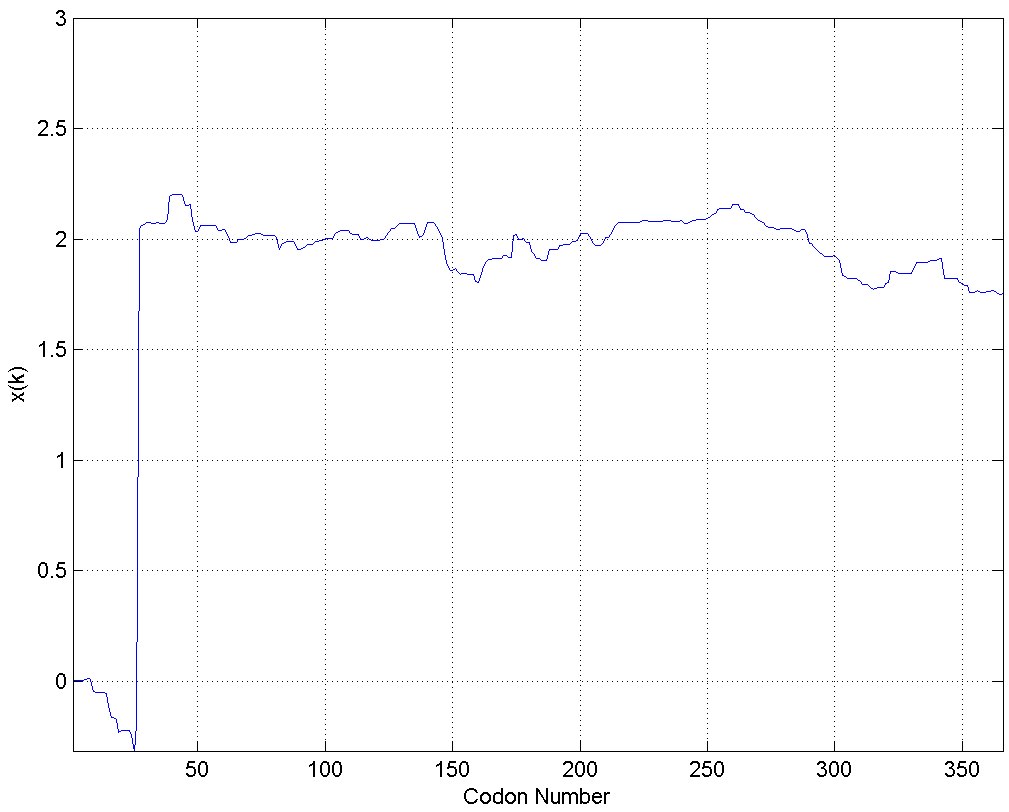
\includegraphics[scale=0.4]{prfB/deterministic}
\end{cfigure}

\begin{wrapfigure}{R}{0.5\textwidth}
  \caption{Polar plot of \prfB}
  \label{prfB:polar}
  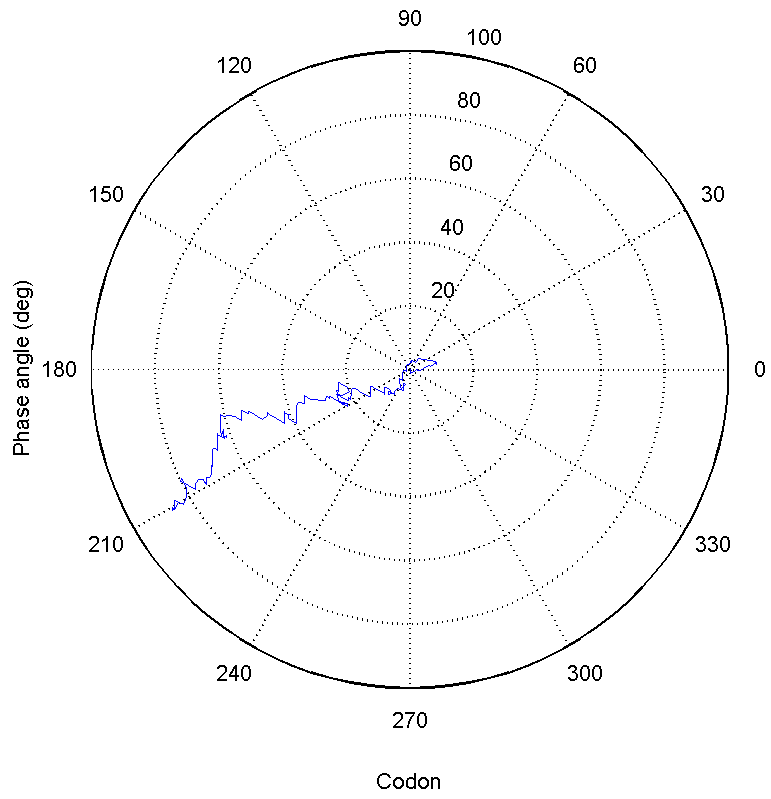
\includegraphics[width=0.5\textwidth]{prfB/polar}
\end{wrapfigure}

First, we let a displacement of $x = 0$ correspond to the zero reading frame and increments of
\emph{two} to represent a one-nucleotide change. For example, $x =2$ represents the +1 frame.
\citet{lalit:embs} prove that both $x = 0$ and $x = 2$ are fixed (stable) points in displacement in their model,
as expected.

A sudden jump from approximately $x = 0$ to $x = 2$ is then the first indication of a $+1$ frameshift.
In essence, this jump suggests that the ribosome skips one entire base pair in the mRNA sequence.
\autoref{prfB:deterministic} shows the displacement plot per this deterministic model for \prfB, 
a gene with a programmed $+1$ frameshift at codon 25.

In conjunction with this characteristic plot, a $+1$ frameshift also displays a clockwise 120\degree\
phase angle rotation from the species angle, consistent with the
creation of the displacement vector from the phasors.
Intuitively, a frameshift sustains if the free energy signal aligns with the sudden jump in displacement.
Since the free energy signal has a period of one codon~\cite{lalit:mechanics}, a $+1$ frameshift the free energy signal
must undergo a phase shift of one-third of an entire period (\autoref{prfB:polar}).

\subsection{A Stochastic Model for Displacement}
\label{stochastic}

As mentioned, the gene \prfB\ exhibits a definite frameshift under the
deterministic model: The displacement jumps to $x=2$.  Certain other
genes, however, demonstrate equivocal, ambiguous behavior near $x = \pm
1$~\cite{lalit:embs}.  In a deterministic model, the fixed
displacement plots implies we cannot clearly interpret whether this
behavior indicates a tendency for a stable frameshift. Even worse,
the model may not show these unstable behaviors at all. In practice,
ribosomal translations are not deterministic. Due to the presence of
noise within the cell environment, any deterministic model ultimately
imperfectly accounts for ribosomal translation especially with regard
to sensitivity to the equivocation of the ribosome between $x=-1$ and
$x=1$. Therefore, we next explored stochastically modeling ribosome
translation with a sinusoidal probability paradigm that follows.

We propose that at each cycle in elongation, the ribosome must make a
decision: stay in the current reading frame, move to the $+1$ reading
frame, or move to the $-1$ reading frame.  We can further subdivide
this choice into the individual wait-cycles.  At each wait cycle, the
ribosome chooses from the above possibilities or proceeds to another
wait-cycle without making a decision.  In addition, we propose that the 
number of wait cycles is inversely proportional to the tRNA availability of 
the codon in the current reading frame, as rarer codons should force the 
ribosome to wait longer for a correct transfer.

Let $abcd$ be a sequence of four nucleotides, with $abc$ in the
current reading frame and $bcd$ in a +1 reading frame.  Let $x$ be the
displacement of the current wait cycle of the ribosome.  As the
incremental displacement approaches +1, the probability of choosing
codon $bcd$ should increase and the probability of choosing codon
$abc$ should decrease.  We model this behavior using even powers of
cosine and sine functions for $abc$ and $bcd$.  We
define $\omega$ as the \emph{weight} that is directly proportional to
the probability.
\begin{equation}
  \omega_{abc} = \cos^{10}{\frac{x\pi}{4}} \text{ and } \omega_{bcd} =
  \sin^{10}{\frac{x\pi}{4}}.
  \footnote{For the purposes of this model, the cosine and sine
    functions are taken to the tenth power, but in future studies,
    this parameter, which must be an even integer, can change.}
\end{equation}
If the ribosome lies completely in the 0 frame, then the probability
of staying in the 0 frame should be 1.  Consequently, if the ribosome
lies fully in the +1 frame ($x=2$), the probability of going to the 0
frame should be 0. Therefore, these functions have a period of two
base pairs ($x=4$).

We also define a value $N_{abc}$ that is the number of wait cycles 
allowed by the given in-frame codon.  Now assume we are at a particular wait cycle. In absence of further
research, we assume by the principle of indifference the probability
of frameshifting is 1/2.  Let $P$ be the instantaneous probability of
moving on to the next codon and staying in the current reading frame.
Then we should have $1-\left(1-P\right)^{N_{abc}} = \frac{1}{2}$.
Given that $P \propto \omega_{abc}$, let $n_{abc}$ be the constant of
proportionality; thus $n_{abc} = \omega_{abc} / P$.  We have
$\omega_{abc} \le 1$, so hence $n \le \sqrt[N]{2}/(\sqrt[N]{2} - 1)$
where $n = n_{abc}$ and $N = N_{abc}$.  Mathematically, the
probability of choosing the codon at a given wait cycle in the zero reading frame is just
\begin{align}
  \prod_{i=1}^K \left(1-\frac{\omega_i}{n}\right) \text{ where } \omega_i = \cos^{10}{\frac{x_i\pi}{4}}.
\end{align}
Here, $n$ represents the wait time for that codon and $K$ is the
ordinal of the current wait cycle. For example, $K=1$ on the first wait
cycle, $K=2$ on the second, and so forth.  Importantly,
$\omega$ is dependent on displacement, which increments after
every wait cycle.

Importantly, we have $\displaystyle\lim_{N\rightarrow\infty} n = N/\ln{2}$, indicating 
that the probability of choosing a codon at a given cycle is directly proportional 
to its tRNA availability, another result that coincides with biological evidence.

\subsection{Measures of Sequence Analysis}

As this model is stochastic, multiple runs (the sample size) of the same sequence must be analyzed.
As such, we propose two metrics for analysis of a number of different runs 
simultaneously. 

\subsubsection{Error-Free Rate}

When studying a
sequence with a programmed frameshift, it measures the percentage of runs 
during which the ribosome chooses the correct codon
at \emph{every} juncture.  For a +1 frameshift, for example, the ribosome must
choose the +1 frame at the frameshift codon and stay in the 0 frame before
and the +1 frame after in order for the run to be a success.

\subsubsection{Displacement Deviation}
\label{section:deviation}

We propose the formula
\begin{equation}
    d = \sqrt{\frac{\sum_i \left(x_i - \beta_i\right)^2}{N}}
\end{equation}
where $\beta_i$ is the predicted reading frame at codon $i$, $x$ is
the displacement at codon $i$, and $N$ is the total number of codons
as a measure of the deviation of the sequence from the expected
reading frame.  Usually $\beta_i = 0$ unless a programmed frameshift
exists as it does for \prfB.  For example, for \prfB\ $\beta_i = 2$
for all $i \geq 25$ because \prfB\ frameshifts at codon 25
\textsc{uga} and the model represents a frameshift with +2
displacement per \autoref{section:frameshifts}.

\subsection{Topics of Analysis}
In order to test our computational model, we ran a number of
experiments to analyze sequences present in the \ecoli\ genome.  This
section explains these investigations.

\subsubsection{\prfB\ and Related Sequences}
As discussed, \prfB\ codes for protein release factor B in \ecoli.
Notably, microbiologists agree that \prfB\ has a programmed frameshift
in the 25$^\textrm{th}$ codon~\cite{weiss87}.  We thus test the
gene \prfB\ to determine whether our model can predict this
frameshift.  We downloaded the nucleotide sequence for \prfB\ from
NCBI's Genbank database.  [Dr. Stomp, do we need a citation for genbank?]

\citet{weiss87} performed a number of biological experiments on
\prfB\ to test how mutations in the sequence would affect the rate of
frameshifting.  They present a total of 35 sequences in their paper,
along with relative measures of translational efficiency.  We ran all
these through our model and correlated them with their error-free rates.
We hypothesize that genes found to frameshift at high rates by
\citeauthor{weiss87} should also show high error-free rates under
our model.

\subsubsection{The \ecoli\ Genome and Ribosomal Proteins}
Microbiologists agree that 


\section{Parameters}
For these plots, we used a species angle of $\theta_{\rm{sp}}
=-30\degree$.

\section{Results}
\subsection{\prfB}

\begin{cfigure}
  \caption{Stochastic displacement plot of \prfB}
  \label{prfB}
  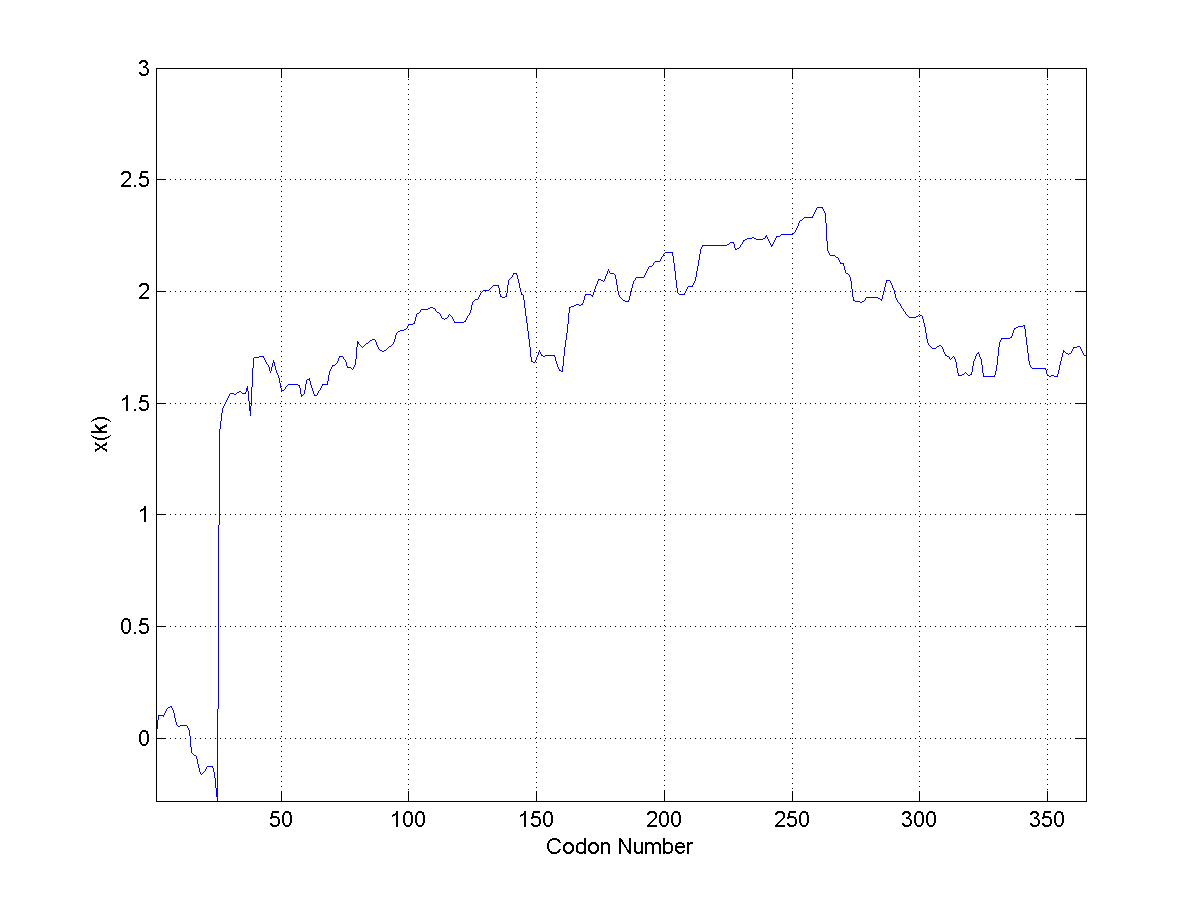
\includegraphics[scale=0.4]{prfB/disp}
\end{cfigure}

In \ecoli, the gene \prfB\ codes for protein release factor B, an
essential element in translation.  This gene, as mentioned, is known
to have a programmed frameshift at the 25$^{\textrm{th}}$ codon.
\autoref{prfB} shows a displacement plot for
\prfB, again with a distinctive jump at codon 25.
\footnote{Note that the polar plot is the the same as \autoref{prfB:polar}. 
The new model does not alter the polar plot or the free energy calculations.}

Notably, the displacement plot does not reach $x=2$ over the span of one codon, as the old model predicted.
Rather, due to randomness, the ribosome chooses the codon in the $+1$ frame before actually reaching a displacement of exactly 2.
The propensity to approach $x=2$, however, concurs with biological
evidence indicating the ribosome stays in frame after the frameshift.
[Dr. Stomp, we need references here.]

\begin{cfigure}
  \caption{Sensitivity plot for \prfB}
  \label{prfB:sens}
  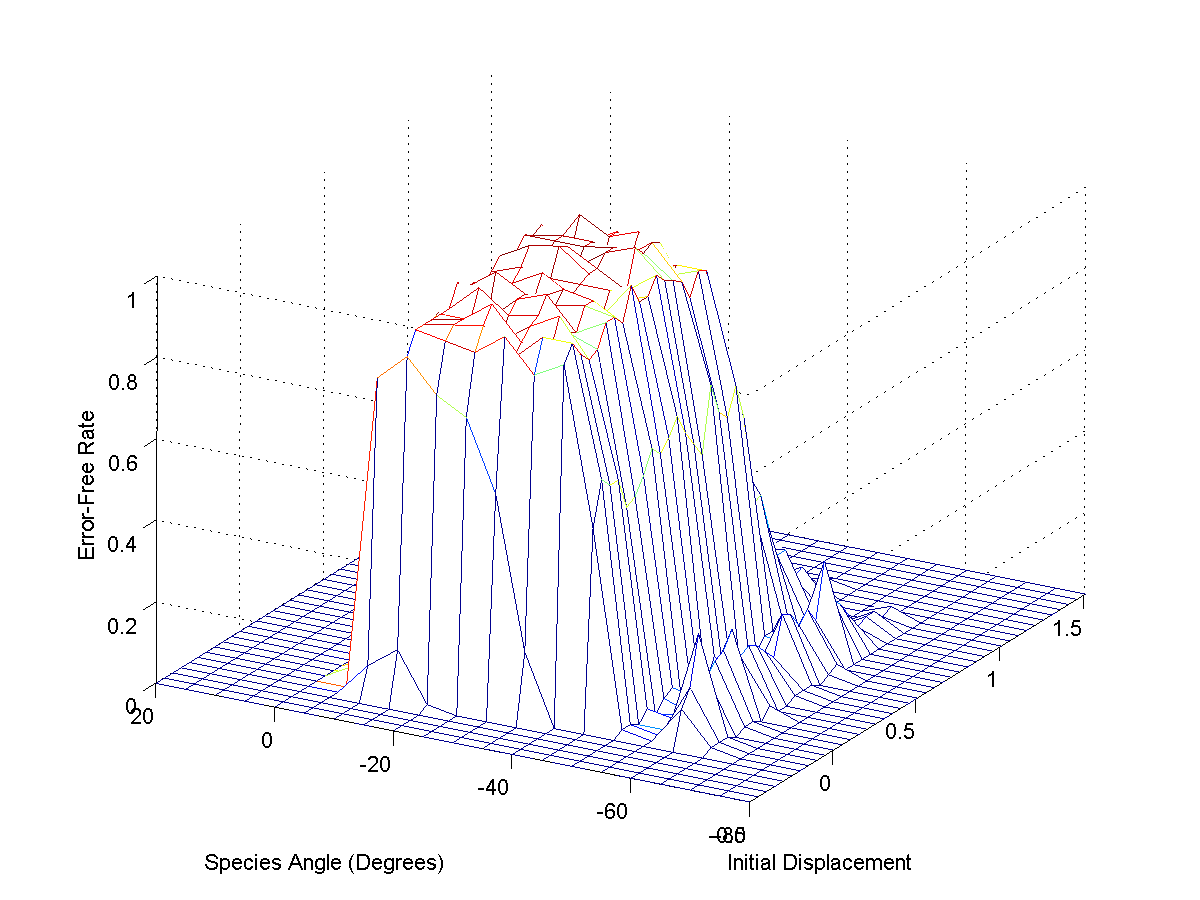
\includegraphics[scale=0.4]{prfB/sensitivity}
\end{cfigure}

We repeated Weiss's experiments computationally
using the stochastic model, and our results agreed~\cite{weiss87,weiss88}.
This concurrence again provides support for the biological validity of
the stochastic model.

Specifically, \citeauthor{weiss87} moved the stop codon in the
\prfB\ sequence one nucleotide upstream, causing the sequence to fail to
frameshift. Moving the stop codon another nucleotide upstream failed
to create a frameshift as well in our model.

\subsection{\ecoli\ genes}
\begin{wrapfigure}{R}{0.55\textwidth}
  \caption{Displacement deviation for \ecoli\ genes with with
    deviation >3 (<1\%) truncated}
  \label{ecoli:hist}
  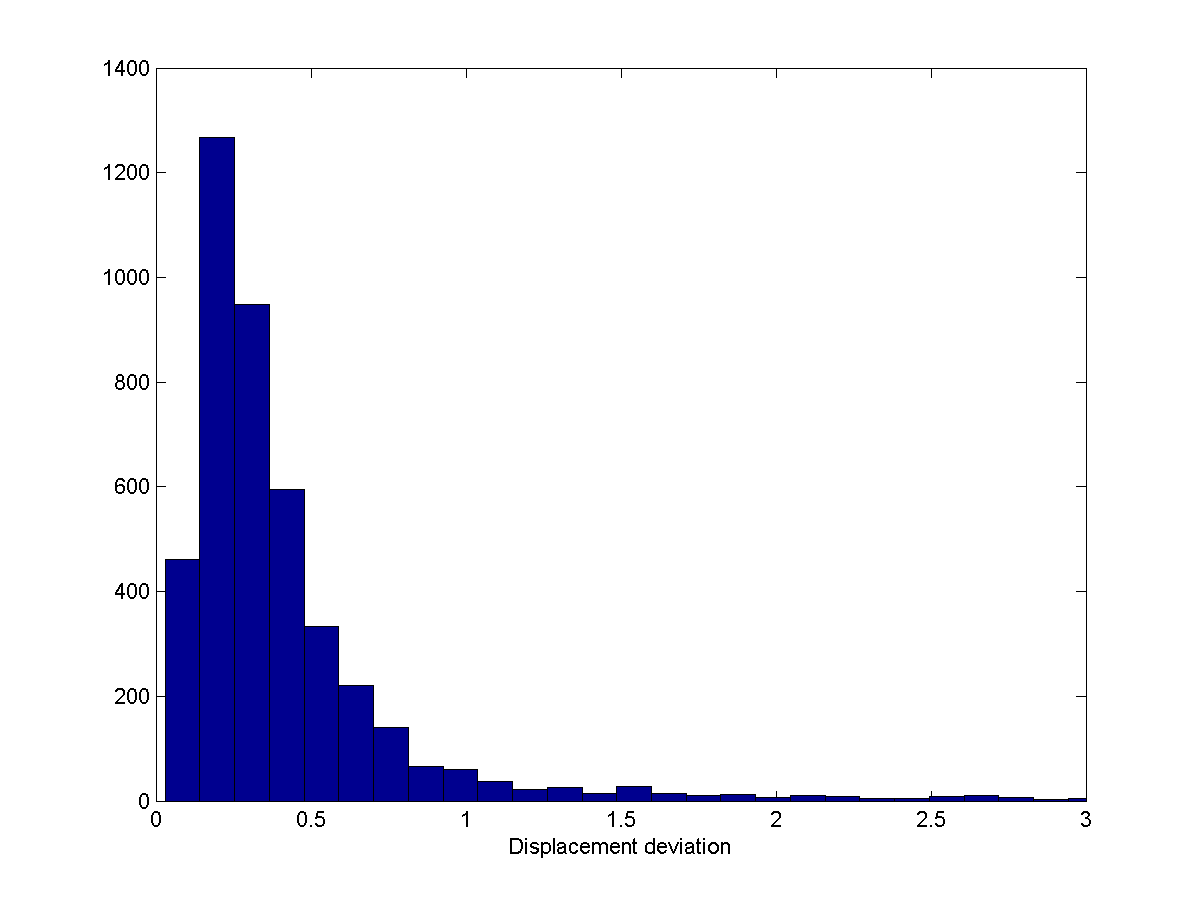
\includegraphics[width=0.55\textwidth]{histograms/everything}
\end{wrapfigure}

\ecoli, as a product of evolution, is naturally efficient in its
processes. [Dr. Stomp, we need references here.]
It logically follows that the model should indicate low deviation
for most \ecoli\ proteins.
\autoref{ecoli:hist} is a histogram of the deviation yields of 4364 genes of
\ecoli, over 80\% of the entire genome.  As predicted, 93.45\% of the genes that we ran
[Guys, expand on this.] laid in the 0 to 1 interval.  The average displacement deviation
for these \ecoli\ genes is [Guys, what?], in a run for 100 iterations per genes.

\subsection{Ribosomal Proteins}
\begin{wrapfigure}{R}{0.3\textwidth}
  \caption{Boxplot comparison of ribosomal proteins and an almost
    complete sample of verified \ecoli\ genes}
  \label{ribosomal:comp}
  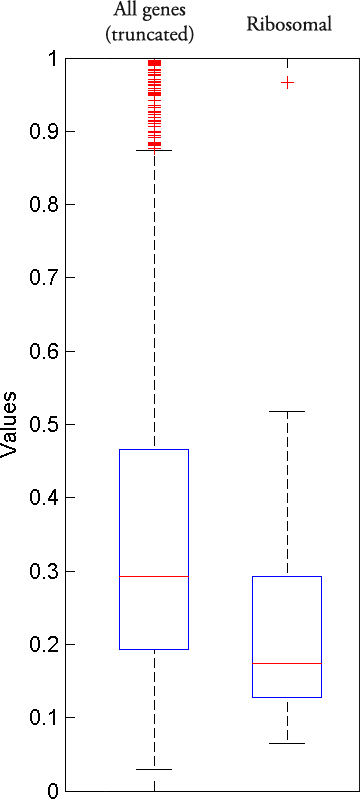
\includegraphics[width=0.3\textwidth]{histograms/ribosomal.png}
\end{wrapfigure}

To compound this finding, biologists also agree that ribosomal
proteins offer especially high translational efficiencies, since the
cell must produce them in such large quantities. [Dr. Stomp, we need
  references here.] The displacement deviation for ribosomal proteins
is in fact [Guys, what?]. We found the average displacement deviation
to be [Guys, what?], which is significantly lower with a $t$-value of
[Guys, what?].

[Guys, outliers.]

\subsection{Bovine Growth Hormone}
\label{section:bgh}

We investigated the concept of deviation yield as a measure of biological
yield by studying bovine growth hormone (bGH), a protein commonly used
in agriculture.
Research~\cite{schoner:bgh} at the time attempted to produce bGH
in \ecoli\ in large amounts.

\begin{tabular}{lccc}
  \toprule
  \textbf{Sequence} & $d$ & $\sigma(d)$ & Yield (\% bGH)\\
  \midrule
  pCZ101 & 0.5146 & 0.03313 & 30 \\
  pCZ105 & 0.5139 & 0.04181 & 34\\
  pCZ112 & 0.6612 & 0.03633 & 33\\
  pCZ115 & 0.6721 & 0.03792 & 32\\
  \midrule
  pCZ100 & 0.7107 & 0.01715 & $<$ 0.5\\
  pCZ104 & 0.7162 & 0.01433 & $<$ 0.5\\
  pCZ108 & 0.5912 & 0.05976 & 1.7\\
  pCZ110 & 0.7026 & 0.01966 & $<$ 0.5\\
  \bottomrule
\end{tabular}


\citet{schoner:bgh}, primarily modifying the initial codons of an
initial bovine growth hormone sequence, found sequences pcZ101,
pcZ105, pcZ112, and pcZ115, to have particularly high protein yield
and to be efficient in comparison to the six other sequences. In
modeling displacement, we found these four sequences  to have the least
displacement deviation from $x = 0$
(\autoref{bgh:deviation}). \autoref{bgh:disp} shows the displacement
plots of all the bGH sequences on the same set of axes. Although not
immediately obvious, the four sequences do indeed indicate lower
deviation. Despite running the genetic algorithm, pcZ108 remains an
outlier because \citeauthor{schoner:bgh} reported low protein
efficiency whereas our model reports low deviation, incongrous with
previously established correlations.

\begin{cfigure}
  \caption{Displacement plot for bGH}
  \label{bgh:disp}
  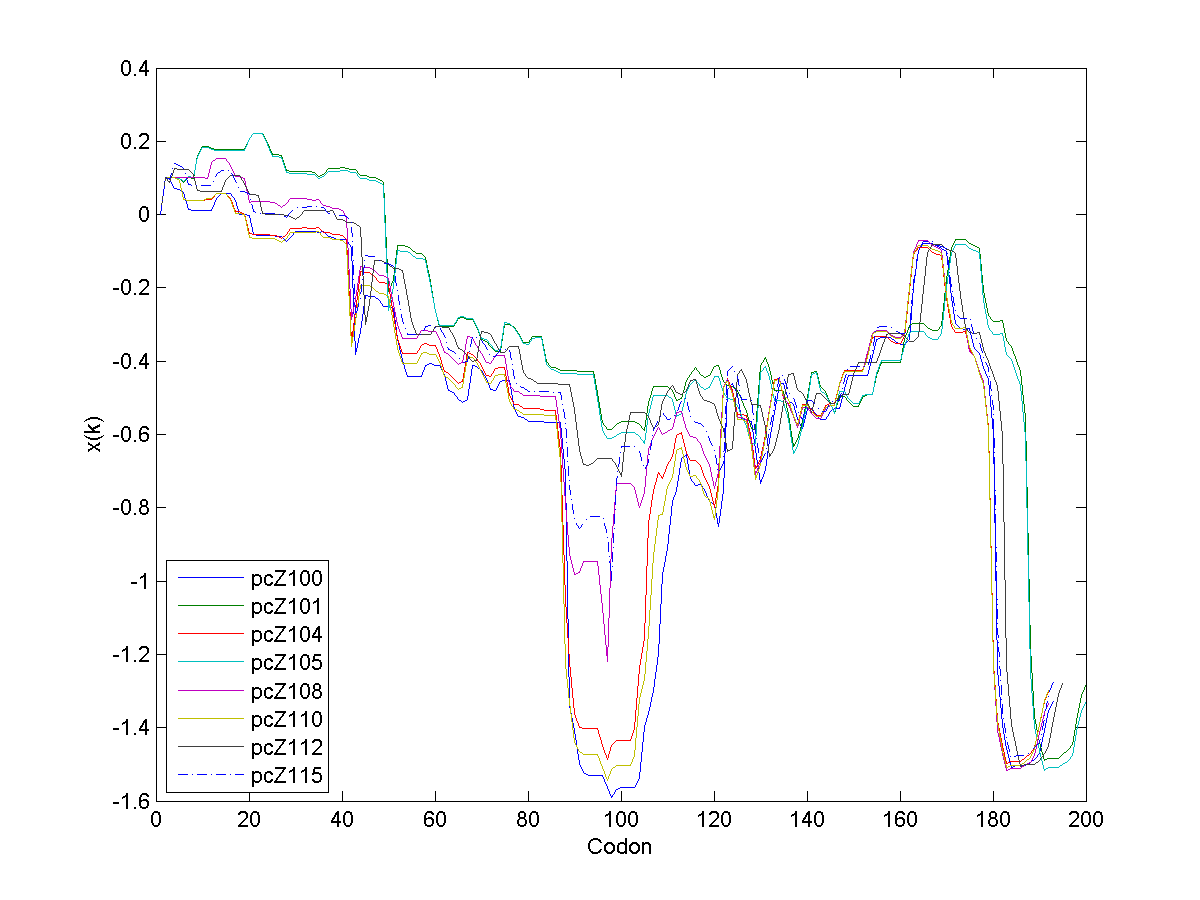
\includegraphics[scale=0.4]{bgh/all}
\end{cfigure}

\subsection{Optimizing Translational Efficiency}

If deviation yield is in fact a potential metric for biological yield,
a method for optimizing deviation would be of use of biologists.  As such,
we wrote an algorithm to minimize deviation for given sequences.
We tested this algorithm computationally on \rpoS, a gene known to
be translationally regulated.  Biological experiments will be
conducted soon.

% I'm colluding deviation and probability yield here, but it's for a
% good purpose. --Hao.

\citet{rpoS:process} indicate that \rpoS, a gene that codes for an RNA
polymerase sigma factor, contains sections of rare codons that disrupt
ribosomal translation. Indeed, our computation model agrees with this
biological evidence, showing again moderately high deviation from $x =
0$. In mass production of such a polymerase sigma factor, biologists
can replace sequences of codons known to add noise and error to
ribosomal translation with synonymous codons. 
However, with a computation model, the process is much
faster and, with this performance, we can perform a randomized, greedy
algorithmic search for codon sequence replacements. We first find an
early trouble spot\footnote{Specifically, places with
  mistake frameshifts in our model, which correlate to rare codons per
  above discussion.} of four codons, randomly replacing that sequence
with synonymous four codons, and running our model against those
permutations to obtain a locally optimal sequence at that place. We
then repeat for all trouble spots the first, terminating when we have locally
optimized the last one. With this algorithm, we reduced our standard
deviation metric for the \rpoS\ displacement plot from 0.168 to 0.117
on sample size of 1000 with a replacement of 33 codons. The
initial correlation between deviation and biological expression
provides strong anecdotal evidence that, with future biological
experimentation, our algorithm has indeed increased protein yield
bypassing a potentially slow biological experimentation process.

[Dr. Stomp, we need the notes that you mentioned.]

\section{Discussion}
Yet, we must note that the model is quite robust; minor changes
in $\theta_{\rm{sp}}$ and initial displacement do not affect frameshifting significantly~\autoref{prfB:sens}.
\autoref{prfB:sens} illustrates the error-free rate as
a function of species angle and initial displacement. As noted,
the frameshift holds over quite a wide range.

Therefore, our model agrees with life in that ribosomal proteins
express much more highly than genes in general.

These results from bovine growth hormone in addition to correlation with a broad
spectrum of known ribosomal behavior indicate our computational model
can significantly increase the speed at which geneticists and
biologists can obtain valuable information when synthesizing
commercially or medicinally useful compounds without laboriously
working through biological experiments.

Our model agrees with his findings.

\phantomsection
\addcontentsline{toc}{section}{References}
\begin{singlespace} \bibliography{wizards} \end{singlespace}
\end{document}
